\documentclass[11pt,a4paper]{article}
\usepackage{amsmath,amssymb,amsthm}
\usepackage{geometry}
\usepackage{hyperref}
\usepackage{booktabs}
\usepackage{parskip}
\usepackage{xcolor}
\usepackage{graphicx}

\geometry{margin=2.5cm}

\newcommand{\E}{\mathbb{E}}
\newcommand{\N}{\mathcal{N}}
\newcommand{\Lcal}{\mathcal{L}}
\newcommand{\R}{\mathbb{R}}
\newcommand{\code}[1]{\texttt{#1}}
\newcommand{\todo}[1]{\textcolor{red}{[TODO: #1]}}

\title{%
  From Pixels to a Periodic Phase Signal:\\
  Per-Shot Kinematic Inference and Its Effect on $(A_s,A_c)$ Recovery
}
\author{}
\date{}

\begin{document}
\maketitle
\tableofcontents
\newpage

%%============================================================
\section{Problem Statement}
\label{sec:problem}
%%============================================================

A gradiometer measures a weak, periodic phase signal $\beta=(A_s,A_c)$ by
repeating a shot $i=0,\dots,N-1$ at a fixed rate, injecting a known
sinusoidal phase modulation
\begin{equation}
  \delta\phi_i(\beta) = A_s\sin(2\pi f i) + A_c\cos(2\pi f i)
  \label{eq:dphi}
\end{equation}
between two atom-interferometer (AI) measurement planes ($z=0$ and
$z=100$), and reading out the result as a pixel-resolved fluorescence image
at each plane. Each shot also carries an independent, a priori unknown
common-mode phase offset $\phi_i\sim\mathrm{Uniform}(0,2\pi)$ (laser phase
noise, not part of the signal), and the atom cloud itself has a shot-dependent
8-dimensional phase-space state $\theta_{iz}$ (mean position/velocity and
Gaussian spread, at plane $z$) that is \emph{not} directly observed --- only
its effect on the recorded image is.

The question this note answers empirically: \textbf{how much does it matter,
for recovering $\beta$, how well $\theta_{iz}$ is estimated from the image?}
We compare four ways of getting $\theta_{iz}$ (from a null guess, to a
prior-art moment estimator, to the best pixel-likelihood estimator developed
in this project, to the oracle/true value), holding the downstream
signal-recovery step fixed, at two photon-count regimes ($10^6$ and $10^8$
atoms per shot). No analytic/Fisher-information arguments are used anywhere
in this note --- every number reported is a direct, empirical
fit-vs.-ground-truth comparison on simulated data with known truth.

%%============================================================
\section{The Reduction: From $(A_s,A_c)$ to Per-Shot $\theta_{iz}$}
\label{sec:reduction}
%%============================================================

This section derives why estimating $\beta$ reduces to (1) a per-shot,
per-plane estimate of $\theta_{iz}$ from the image, followed by (2) a
signal-fit step that takes those estimates (and per-shot photon counts) as
input. The notation matches \code{notes/joint\_profile\_inference.tex}
(``Per-Shot Pixel Likelihood'' section there) exactly.

\paragraph{Scope of the reduction, stated up front.} Two facts below are
\emph{exact} regardless of how the image is read out: the per-shot phase
$\phi_i$ is a single scalar nuisance shared across both planes
(\S\ref{sec:step1}), and $\beta$ enters \emph{only} through the scalar
$\delta\phi_i(\beta)$ (\S\ref{sec:step2}). Two further steps are
\emph{approximations}, and it is important not to conflate them with the
exact structure:
\begin{enumerate}
  \item \textbf{Plug-in $\theta$.} Eq.~\ref{eq:beta-mle} fixes $\theta$ at a
    per-shot point estimate $\hat\theta_{iz}$ and maximises over $\beta$,
    rather than marginalising $\theta$ against its posterior. This is exact
    only in the sharp-$\theta$-posterior (high photon-count) limit; in
    general it discards the ($\beta$-dependent) width of the
    $\theta$-posterior.
  \item \textbf{Position averaging.} As \emph{implemented}
    (\code{map\_inference.py}'s \code{total\_logL\_fast}\,/\,%
    \code{\_ai\_ll\_batch}), the signal-fit step uses only the
    \emph{port-summed total counts} $(n_g,n_e)$ per plane against the
    \emph{spatially-integrated} coherence coefficients $(A,C^c,C^s)$ --- i.e.\
    a two-bin (port-$g$/port-$e$) Poisson likelihood per plane, not the full
    pixel-resolved image likelihood. See \S\ref{sec:whatimplemented} for why
    this is \emph{not} the same as the full-image likelihood, and $\hat\theta$
    is \emph{not} a sufficient statistic for $\beta$.
\end{enumerate}
In other words, the clean statement ``$\beta$-fit needs only $\hat\theta$ and
counts, not the images'' is a property of the \emph{position-averaged}
(port-population) model that this pipeline actually uses --- it is not a
lossless reduction of the full-image likelihood.

\subsection{The observation model}

At AI $z$, pixel $b$, detection state $s\in\{g,e\}$, shot $i$:
\begin{equation}
  n_{izsb} \sim \mathrm{Poisson}\bigl(\lambda_{izsb}\bigr), \qquad
  \lambda_{izsb} = L_{iz}\Bigl[A_{sb}(\theta_{iz}) + C^c_{sb}(\theta_{iz})\cos\Phi_{iz}
                                                    + C^s_{sb}(\theta_{iz})\sin\Phi_{iz}\Bigr],
  \label{eq:obs-model}
\end{equation}
where $\Phi_{iz} = \phi_i + \delta\phi_i(\beta)\cdot[z{=}100]$ is the total
phase seen at plane $z$, $(A,C^c,C^s)$ are the PSMAP-model coherence
coefficients (Gaussian-cloud-averaged atom optics response, a deterministic
function of $\theta_{iz}$ only -- see the ``Pixel ACS'' section of
\code{joint\_profile\_inference.tex}), and $L_{iz}$ is a total-count
normalisation fixed by the data (same reference, ``Objective Rescaling''
recap equation), not a free parameter.

\subsection{Step 1: the nuisance phase is a per-shot, per-plane-pair
quantity}
\label{sec:step1}

$\phi_i$ appears \emph{identically} in both planes' $\Phi_{iz}$ (shifted by
the known $\delta\phi_i(\beta)$ at $z{=}100$) -- it is a single scalar
nuisance per shot, not per plane. Marginalising it out of the per-shot
likelihood,
\begin{equation}
  p(n_{i,0},n_{i,100}\mid\theta_{i,0},\theta_{i,100},\beta)
  = \int_0^{2\pi} p(n_{i,0}\mid\theta_{i,0},\phi_i)\,
              p(n_{i,100}\mid\theta_{i,100},\phi_i+\delta\phi_i(\beta))\;
              \frac{d\phi_i}{2\pi},
  \label{eq:marginal-phi}
\end{equation}
gives the shot's \emph{marginal} log-likelihood as a function of
$(\theta_{i,0},\theta_{i,100},\beta)$ alone -- $\phi_i$ never needs to be
reported or stored once this integral is done. This is a 1-dimensional,
periodic, and (empirically, this project) cheap-to-integrate-numerically
nuisance -- see \S\ref{sec:phi-marginal-method} for how it is done in
practice.

\subsection{Step 2: $\beta$ enters \emph{only} through $\delta\phi_i(\beta)$,
which is known given $\theta$}
\label{sec:step2}

For \emph{fixed} $\theta_{i,0},\theta_{i,100}$, the marginal likelihood
(Eq.~\ref{eq:marginal-phi}) is a function of $\beta$ \emph{only} through the
scalar $\delta\phi_i(\beta)$ -- a known, linear-in-$\beta$ function of the
shot index $i$ (Eq.~\ref{eq:dphi}). This is the entire mechanism by which
repeated shots pin down $(A_s,A_c)$: each shot supplies one (generally weak,
individually) constraint on $\delta\phi_i(\beta)$, and because
$\delta\phi_i(\beta)$ traces out a known sinusoid in $i$, combining $N$
shots' constraints via
\begin{equation}
  \hat\beta = \arg\max_\beta \sum_{i=0}^{N-1}
    \log p\bigl(n_{i,0},n_{i,100}\mid\hat\theta_{i,0},\hat\theta_{i,100},\beta\bigr)
  \label{eq:beta-mle}
\end{equation}
recovers $\beta$ with a precision that improves with $N$ (standard harmonic
regression). The entire image-processing burden is front-loaded into
estimating $\theta_{iz}$ per shot, and every method compared in this note
differs \emph{only} in how that front-loaded estimate is produced. What
information the signal-fit likelihood in Eq.~\ref{eq:beta-mle} actually
consumes -- the full pixel-resolved image, or a position-averaged summary
of it -- is the subject of \S\ref{sec:whatimplemented}, and matters for how
lossless the reduction is.

\subsection{The reduction, stated plainly}

\begin{quote}
\emph{Estimating the periodic signal $(A_s,A_c)$ from $N$ shots of
pixel-resolved images reduces to: (a) for each shot and each plane,
estimate the 8-dimensional cloud state $\theta_{iz}$ from that single
image (after marginalising the shot's own unknown common phase $\phi_i$);
then (b) fit $\beta$ against the known sinusoidal structure of
$\delta\phi_i(\beta)$, using only the per-shot $\hat\theta_{iz}$ and raw
photon counts as input.}
\end{quote}

This is why the four methods compared below (\S\ref{sec:methods}) differ
\emph{only} in step (a) -- step (b) (Eq.~\ref{eq:beta-mle}, implemented via
\code{map\_inference.py}'s \code{batch\_acs\_gh} + \code{total\_logL\_fast}
pipeline) is held \emph{identical} across all four, so any difference in
the resulting $\hat\beta$ is attributable entirely to the quality of the
per-shot kinematic estimate.

\subsection{What step (b) actually consumes: a port-population likelihood,
not the full image}
\label{sec:whatimplemented}

The reduction quoted above is exact as a \emph{structural} statement (Steps
1--2), but the phrase ``uses only $\hat\theta$ and raw counts, not the
images'' hides a modelling choice that is worth stating precisely, because
it makes the reduction lossy at the full-image level.

\paragraph{What is implemented.} The signal-fit likelihood
(\code{total\_logL\_fast} $\to$ \code{\_ai\_ll\_batch}) evaluates, per shot
and per plane, a \emph{two-bin Poisson} likelihood in the total port counts
$(n_g,n_e)=\bigl(\sum_b n_{izgb},\ \sum_b n_{izeb}\bigr)$ against
\emph{spatially-integrated} coefficients
$\bigl(A_s,C^c_s,C^s_s\bigr)=\sum_b\bigl(A_{sb},C^c_{sb},C^s_{sb}\bigr)$
(the six numbers returned by \code{batch\_acs\_gh} per shot). The
pixel-resolved image $n_{izsb}$ enters the pipeline \emph{only} through the
upstream estimate $\hat\theta_{iz}$; it never appears in the $\beta$-fit
itself. This is a \emph{position-averaged} (port-population) likelihood.

\paragraph{Why this is not the full-image likelihood.} In the observation
model (Eq.~\ref{eq:obs-model}) the phase enters through
\emph{pixel-dependent} fringe coefficients $C^c_{sb}(\theta)$,
$C^s_{sb}(\theta)$: the signal phase $\Phi_{iz}$ (hence $\delta\phi_i(\beta)$,
hence $\beta$) modulates the \emph{spatial pattern}, not merely the per-port
totals. Summing over pixels to form $(n_g,n_e)$ keeps only the projection
$\sum_b C^c_{sb}$ (one number per port) and discards the rest of the fringe's
$\beta$-dependence. Consequently:
\begin{itemize}
  \item $\hat\theta_{iz}$ is \textbf{not} a sufficient statistic for
    $\beta$: there is no factorisation theorem here, and indeed $\hat\theta$
    is estimated \emph{after} marginalising $\phi_i$
    (Eq.~\ref{eq:marginal-phi}), so by construction it carries essentially
    no phase information. The $\beta$-information and the $\theta$-information
    live in different features of the image.
  \item The full-image profile likelihood
    $\prod_i p\bigl(\{n_{izsb}\}\mid\hat\theta_{iz},\beta\bigr)$ ---
    i.e.\ Eq.~\ref{eq:beta-mle} taken literally, with the full pixel image
    rather than the port totals --- would additionally exploit the
    pixel-resolved fringe, and is therefore (weakly) \emph{more} informative
    about $\beta$ than the port-population fit this note uses. How much is
    left on the table depends on how strongly $C^c_{sb},C^s_{sb}$ vary across
    pixels relative to their integrals; it is not quantified here.
\end{itemize}

\paragraph{Where the reduction \emph{is} clean.} For the position-averaged
model that is actually run, the statement ``estimate $\theta$ from the image,
then fit $\beta$ from the port counts'' is self-consistent and (up to the
plug-in-$\theta$ approximation of \S\ref{sec:reduction}) exact: the port
populations depend on $\beta$ only through $\delta\phi_i(\beta)$ and the
$\theta$-dependent integrated coefficients, exactly as Eq.~\ref{eq:beta-mle}
uses them. The caveat is only that this port-population likelihood is a
deliberately averaged view of the data, so the comparison in this note is
between kinematic estimators \emph{holding that averaged signal-fit fixed} ---
it does not claim to have extracted every bit of $\beta$-information the full
images contain.

%%============================================================
\section{Methods Compared}
\label{sec:methods}
%%============================================================

All four methods below take one shot's pixel image (at one plane $z$) and
return an estimate $\hat\theta_{iz}\in\R^8$; nothing else in the pipeline
changes between them.

\subsection{Null (uninformative baseline)}
\[
  \hat\theta_{iz}^{\rm null} = \bar\theta \quad\text{(the prior mean, every shot, always)}.
\]
Uses \emph{no} image information whatsoever. This is the floor any real
method must beat, and (since it never varies) it directly shows what
$\hat\beta$ looks like when the signal-fit step (Eq.~\ref{eq:beta-mle}) is
handed a fixed, uninformative, shot-independent guess for $\theta$ at every
shot -- isolating how much of the ultimately-recovered $\beta$ precision, if
any, survives with zero per-shot kinematic information.

\subsection{MAP-moments (prior art, \code{map\_inference.py})}
\label{sec:map-moments}
The existing pipeline: reduce the image to its first two port-summed
spatial moments $(\hat\mu_{xf},\hat\mu_{yf},\hat V_{xf},\hat V_{yf})$, then
apply the closed-form Kalman-gain MAP update
$\hat\eta = \bar\eta + K(\hat M - A\bar\eta)$ (Eq.\ in
\code{map\_inference.py}'s \code{map\_eta}) mapping the 4 observed moments
to the 10-dimensional free-flight state $\eta$ (position/velocity means +
full covariance, including a cross term $C_{xv0}$ that $\theta$ does not
have). For comparison against the other three methods' $\theta$
representation, $\eta$ is projected down to $\theta$ by taking
$(\mu_{x0},\mu_{y0},\mu_{vx0},\mu_{vy0})$ directly and
$\sigma_\bullet=\sqrt{V_\bullet}$ for the four spread components, discarding
the estimated cross-covariance terms (which $\theta$-based methods do not
attempt to estimate at all, and which the true generative model sets to
zero exactly). This is a MAP point estimate under a Gaussian
approximation to the moment likelihood -- it explicitly does \emph{not} use
any pixel structure beyond the first two spatial moments.

\subsection{Pixel-likelihood, best configuration}
\label{sec:phi-marginal-method}
The method developed over the course of this investigation: marginalise
$\phi_i$ by \emph{direct numerical quadrature} over a dense grid
($M=2000$ points, verified converged to $\sim10^{-9}$ absolute by varying
$M$ from 500 to 8000 -- \S\ref{sec:qconv}), then optimise $\theta_{iz}$
(8-dimensional) against the resulting smooth marginal log-likelihood via
plain L-BFGS-B (\code{scipy.optimize.minimize}), with the model's own
per-$\phi$-grid-point analytic-ish gradient (from
\code{pixel\_acs\_grad.pixel\_acs\_and\_grad}) chained through the
log-sum-exp marginalisation to give an efficient gradient for the outer
$\theta$-optimisation (\S\ref{sec:analytic-grad}). This inverts the naive
computational order (fix $\phi$, optimise $\theta$ conditionally at every
grid point) that was found, over an extended debugging effort, to
\emph{not} converge reliably at $10^8$ atoms -- see
\code{notes/joint\_profile\_inference.tex}'s ``2026-07-20'' section for the
full negative result this reframing supersedes.

\textbf{Best configuration, established empirically (\S\ref{sec:hp}):}
\begin{itemize}
  \item \code{bins=32} (pixel grid resolution for the image binning)
  \item \emph{tightened} image range: $\pm 1.54\,$mm instead of the
    dataset's native $\pm 3\,$mm, set by the 99.99\%-flux-containment
    radius measured across all 40 available runs (\S\ref{sec:tightrange}) --
    essentially free (same bin count, same evaluation cost), and found to
    give a comparable improvement to doubling the bin count, but at
    $\sim\!1/4$ the compute cost.
  \item \code{pixel\_n\_gh=8} (2D Gauss--Hermite velocity-quadrature order;
    verified converged, no measurable effect from 4 to 16).
\end{itemize}

\subsection{Oracle}
\[
  \hat\theta_{iz}^{\rm oracle} = \theta_{iz}^{\rm true} \quad\text{(read directly from simulation metadata)}.
\]
Represents the shot-noise floor: the best any $\theta$-based pipeline could
possibly do, since it has zero kinematic estimation error and only the
signal-fit step's own Poisson noise remains.

%%============================================================
\section{Experimental Setup}
\label{sec:setup}
%%============================================================

\begin{center}
\begin{tabular}{@{}lp{10cm}@{}}
\toprule
Quantity & Value \\
\midrule
Datasets & $10^6$ atoms/shot (\code{R80\_N200\_A1000000\_...}), $10^8$ atoms/shot (\code{R40\_N50\_A100000000\_...}) \\
Runs per dataset & 10 independent runs (different noise realisations of the same $\beta$) \\
Shots per run & 50 (matched across both atom counts, apples-to-apples) \\
Signal frequency & $f=0.3$ (cycles/shot) \\
True signal & $A_s=0.08776$, $A_c=0.04794$ (same for both datasets) \\
Prior & $\bar\theta=(0,0,0,0,100,100,100,100)\,\mu$m(/s), $\sigma_\theta=10\,\mu$m(/s) per component \\
Best-config bins & 32, image half-range 1.54\,mm (native: 3.0\,mm) \\
Signal-fit ($\beta$) pixel grid & bins=16, native full range, \code{gh\_order=12} (unchanged across all 4 methods) \\
\bottomrule
\end{tabular}
\end{center}

Full derivations of the hyperparameter choices (\code{bins=32}, tight
range, quadrature order) are given in Appendix~\ref{sec:hp}--\ref{sec:qconv}.

%%============================================================
\section{Results}
\label{sec:results}
%%============================================================

\subsection{Kinematic parameter recovery}

Figures~\ref{fig:res1e6}--\ref{fig:res1e8} show the pooled residual
distributions (estimate $-$ truth, both AI planes, all 10 runs $\times$ 50
shots $=$ 1000 samples per method) for all 8 kinematic parameters, at both
atom counts. Table~\ref{tab:theta-rmse} gives the corresponding RMSE.

\begin{figure}[htbp]
  \centering
  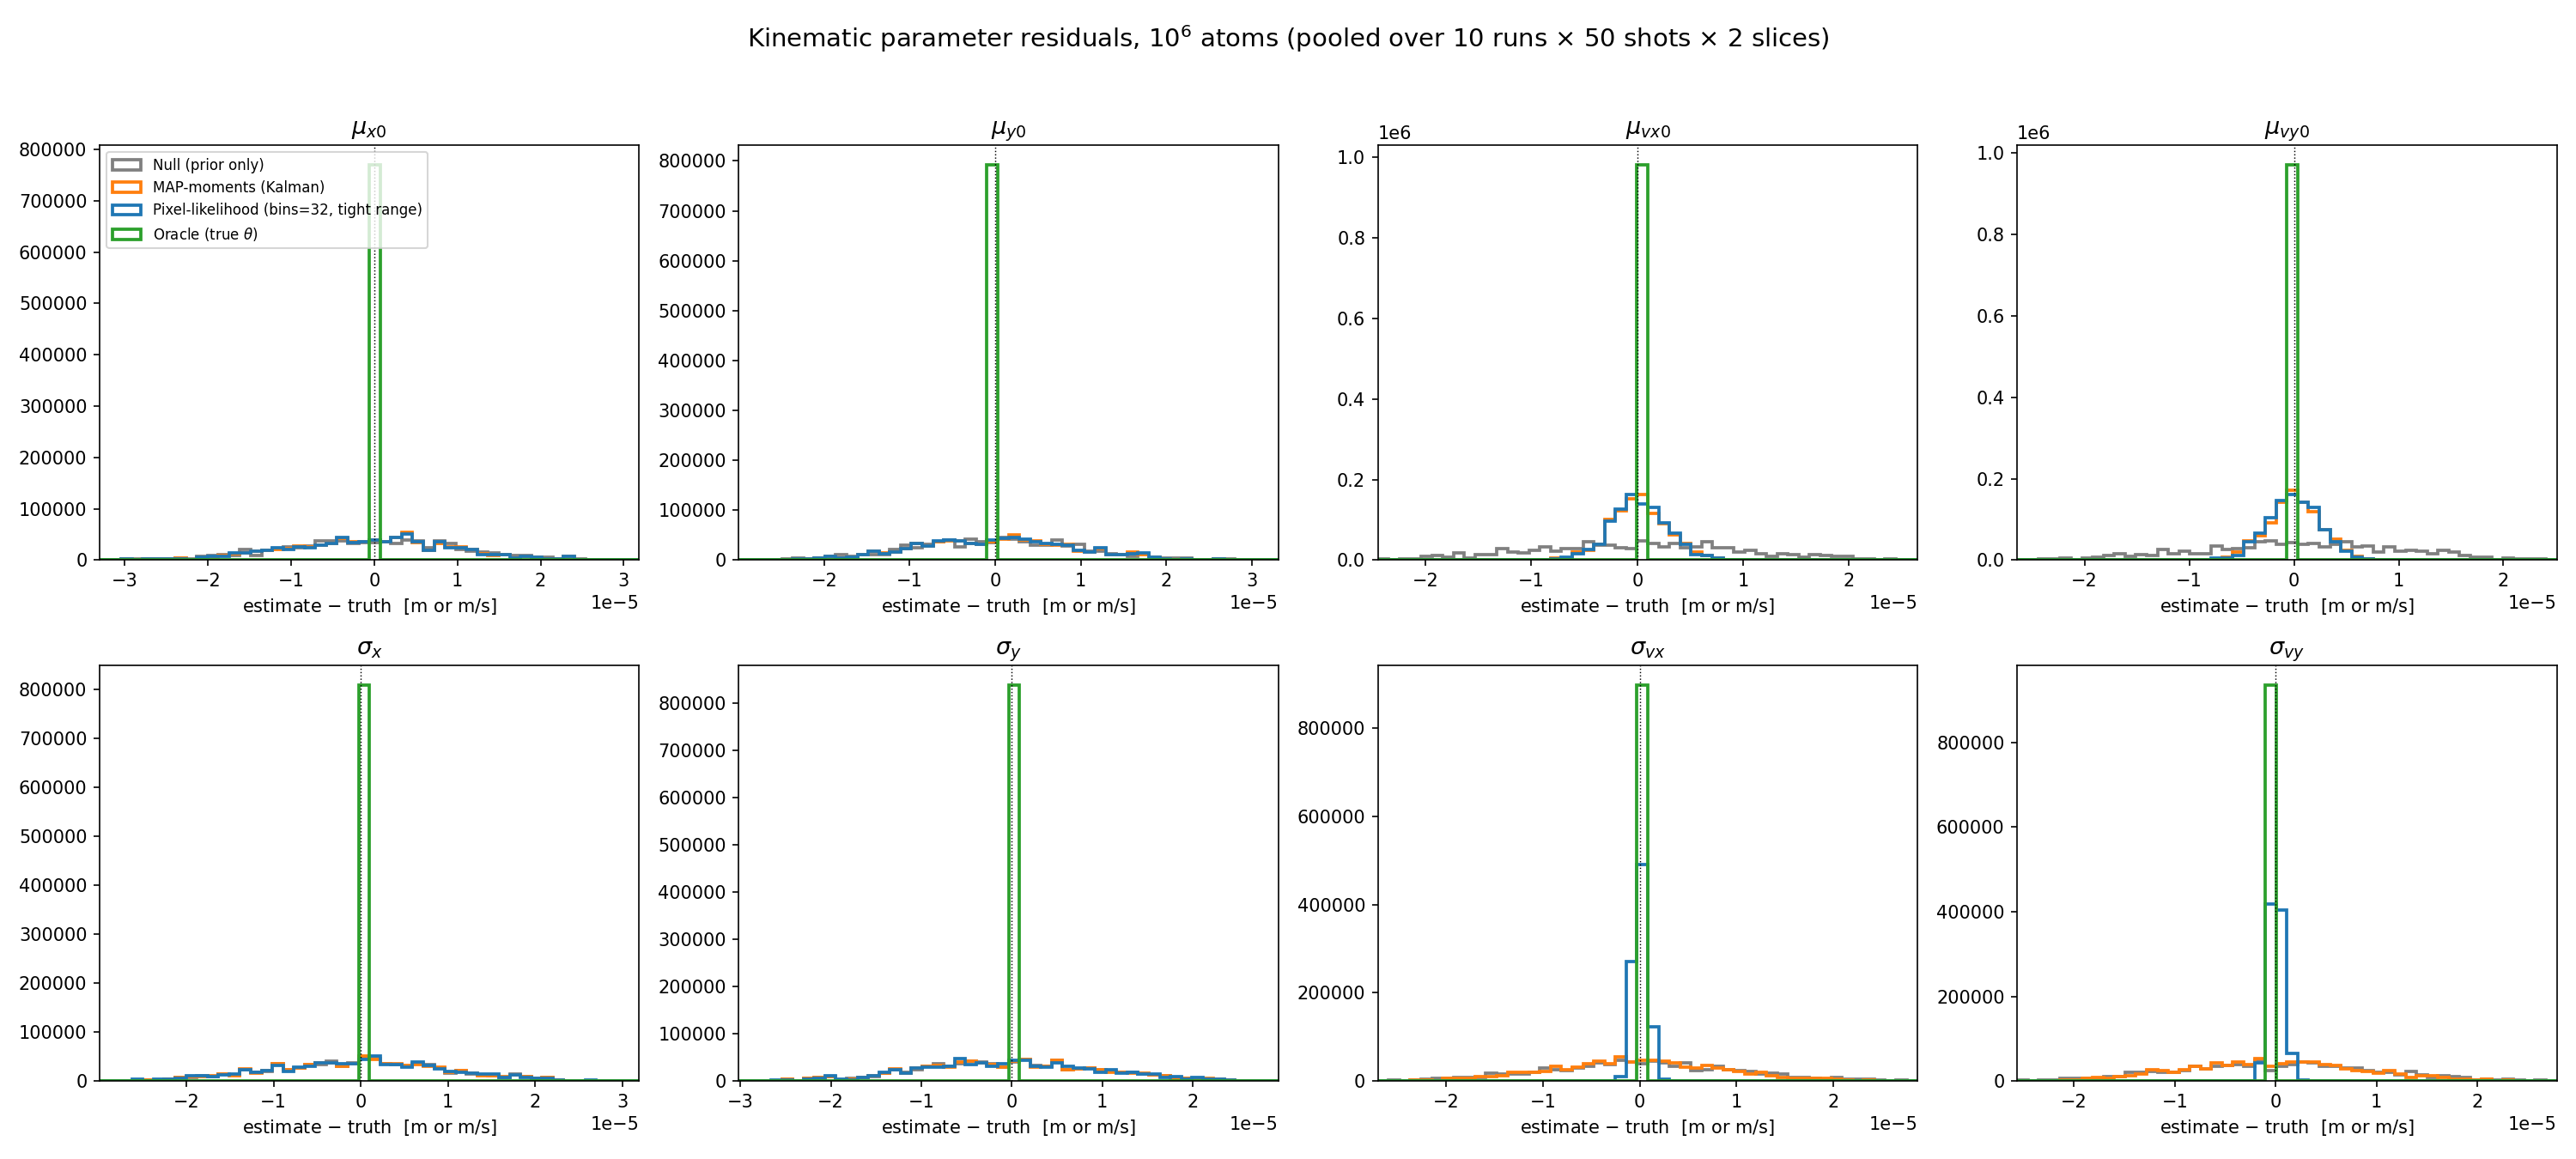
\includegraphics[width=\textwidth]{figures/residuals_1e6.png}
  \caption{Kinematic parameter residuals, $10^6$ atoms.}
  \label{fig:res1e6}
\end{figure}

\begin{figure}[htbp]
  \centering
  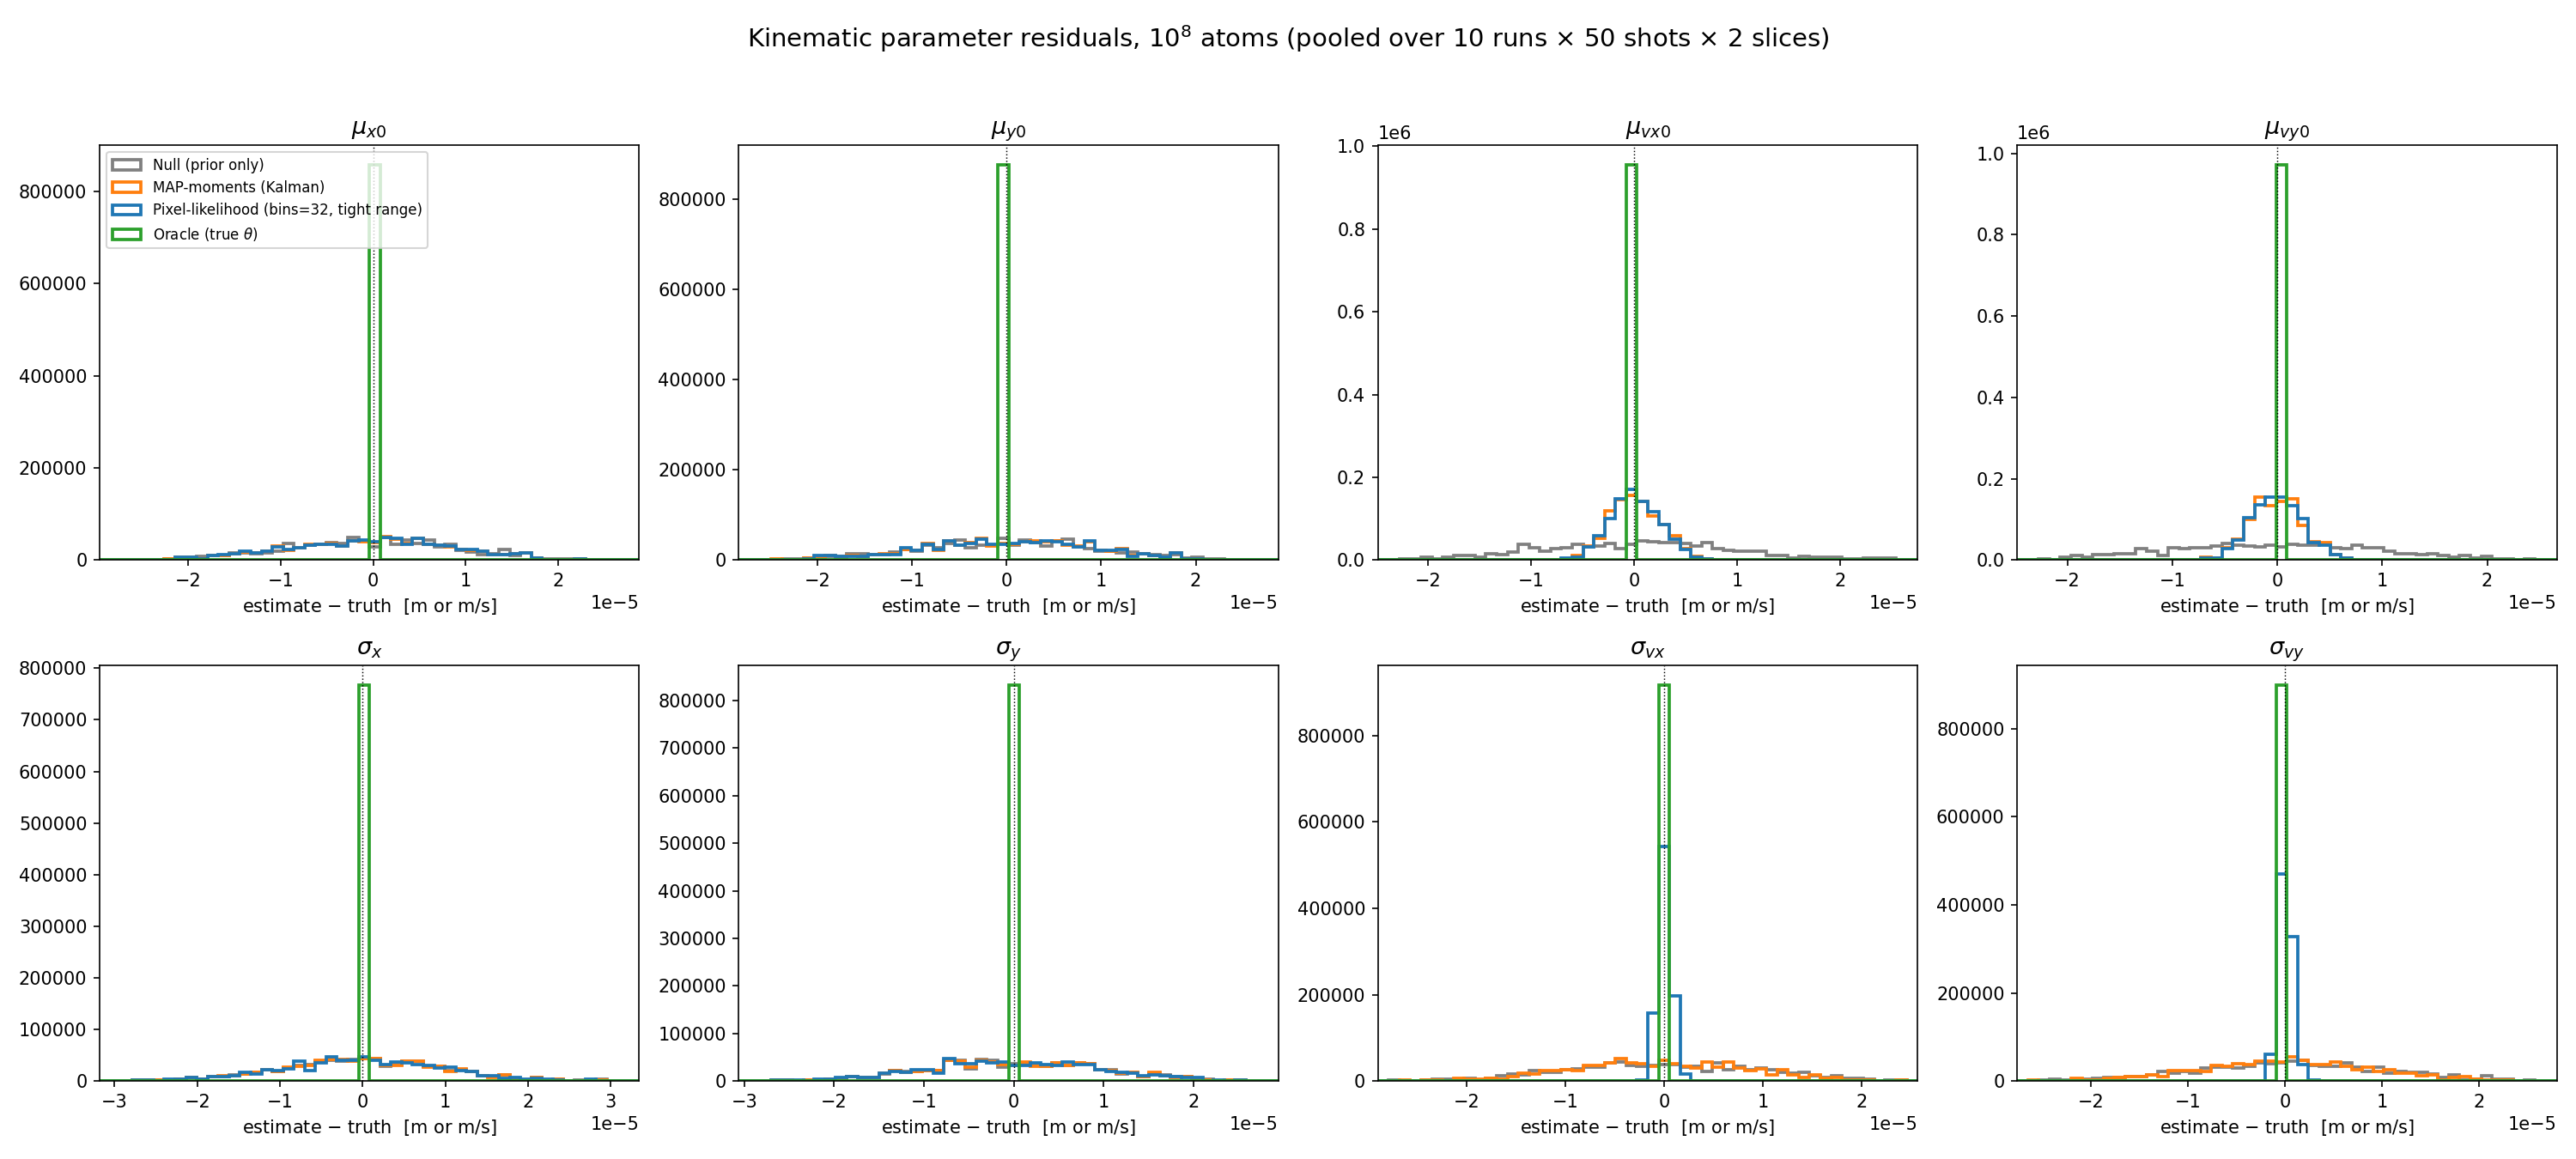
\includegraphics[width=\textwidth]{figures/residuals_1e8.png}
  \caption{Kinematic parameter residuals, $10^8$ atoms.}
  \label{fig:res1e8}
\end{figure}

\begin{table}[htbp]
\centering
\caption{Kinematic parameter RMSE by method and atom count, in
$\mu$m ($\mu_{x0},\mu_{y0},\sigma_x,\sigma_y$) or $\mu$m/s
($\mu_{vx0},\mu_{vy0},\sigma_{vx},\sigma_{vy}$). Position
($\mu_{x0},\mu_{y0}$) and position-spread ($\sigma_x,\sigma_y$) are
essentially unaffected by which method is used -- all three real methods
sit close together, well above the (zero, by construction) oracle. Velocity
mean ($\mu_{vx0},\mu_{vy0}$) shows a moderate, atom-count-independent
advantage for moments/best over null. Velocity spread
($\sigma_{vx},\sigma_{vy}$) is where the pixel-likelihood method's
advantage is concentrated: roughly a $12$--$13\times$ tighter RMSE than
moments, at \emph{both} atom counts.}
\label{tab:theta-rmse}
\begin{tabular}{lrrrr}
\toprule
& \multicolumn{2}{c}{$10^6$ atoms} & \multicolumn{2}{c}{$10^8$ atoms} \\
Parameter & moments & best & moments & best \\
\midrule
$\mu_{x0}$ [$\mu$m]        & $10.17$ & $10.17$ & $9.28$ & $9.28$ \\
$\mu_{y0}$ [$\mu$m]        & $9.68$  & $9.68$  & $9.30$ & $9.29$ \\
$\mu_{vx0}$ [$\mu$m/s]     & $2.70$  & $2.64$  & $2.48$ & $2.40$ \\
$\mu_{vy0}$ [$\mu$m/s]     & $2.56$  & $2.50$  & $2.47$ & $2.41$ \\
$\sigma_x$ [$\mu$m]        & $10.19$ & $10.19$ & $9.87$ & $9.88$ \\
$\sigma_y$ [$\mu$m]        & $10.00$ & $9.99$  & $9.83$ & $9.82$ \\
$\sigma_{vx}$ [$\mu$m/s]   & $8.92$  & $\mathbf{0.705}$ & $8.91$ & $\mathbf{0.670}$ \\
$\sigma_{vy}$ [$\mu$m/s]   & $8.83$  & $\mathbf{0.691}$ & $8.97$ & $\mathbf{0.673}$ \\
\bottomrule
\end{tabular}
\end{table}

The pattern is remarkably consistent across the $100\times$ change in atom
count: the pixel-likelihood method's advantage over moments is
\emph{entirely} concentrated in the two velocity-spread components, at a
roughly constant $\sim\!12$--$13\times$ RMSE reduction regardless of photon
budget.

\paragraph{Checking the mechanism directly, rather than assuming it.} A
first hypothesis was that this concentrates on velocity spread because the
moment method only observes the detection-plane position variance
$V_{xf}=V_{x0}+2T C_{xv0}+T^2 V_{vx0}$, a single scalar mixing three
unknowns -- predicting that moments' $\sigma_x$ and $\sigma_{vx}$
\emph{errors} should be anti-correlated (trading off against each other to
keep $V_{xf}$ fixed). Figure~\ref{fig:res2d1e8} tests this directly by
plotting the joint residual distribution for exactly this pair (and the
analogous mean-parameter pair), per method. \textbf{The na\"ive trade-off
hypothesis is wrong for moments}: $(\sigma_x,\sigma_{vx})$ residuals are
essentially uncorrelated for moments (Pearson $r=-0.06$ at $10^8$ atoms,
$-0.04$ at $10^6$) -- moments' large $\sigma_{vx}$ error is not a
correlated trade-off against $\sigma_x$, it is simply weakly constrained
and close to independent prior-dominated noise. What \emph{is} true, and
turns out to be the more informative finding: the pixel-likelihood method's
$(\sigma_x,\sigma_{vx})$ residuals are almost perfectly anti-correlated
($r=-0.99$, both atom counts) -- and the same near-perfect anti-correlation
appears for the mean pair $(\mu_{x0},\mu_{vx0})$ for \emph{both} methods
($r=-0.97$ moments, $r{\approx}{-1.00}$ best). This is the signature of a
genuinely well-constrained detection-plane observable (approximately
$\mu_{xf}\approx\mu_{x0}+T\mu_{vx0}$, and analogously for the variance):
a good estimator's errors in the two initial-state components must move
oppositely to keep the well-determined combination correct, concentrating
residual uncertainty in the orthogonal, genuinely underdetermined direction.
Moments shows this structure clearly for the \emph{mean} pair but not the
\emph{spread} pair; the pixel-likelihood method shows it clearly for
\emph{both} -- i.e., the moment method fails to extract the (nonlinear,
quadratic-in-cloud-parameters) $V_{xf}$ constraint at all, while the pixel
likelihood recovers it about as well as it recovers the (linear) $\mu_{xf}$
constraint. This is a more precise, and different, explanation than the
originally-hypothesized simple trade-off, and was only established by
checking the correlation structure directly rather than assuming it from
the model equations.

\begin{figure}[htbp]
  \centering
  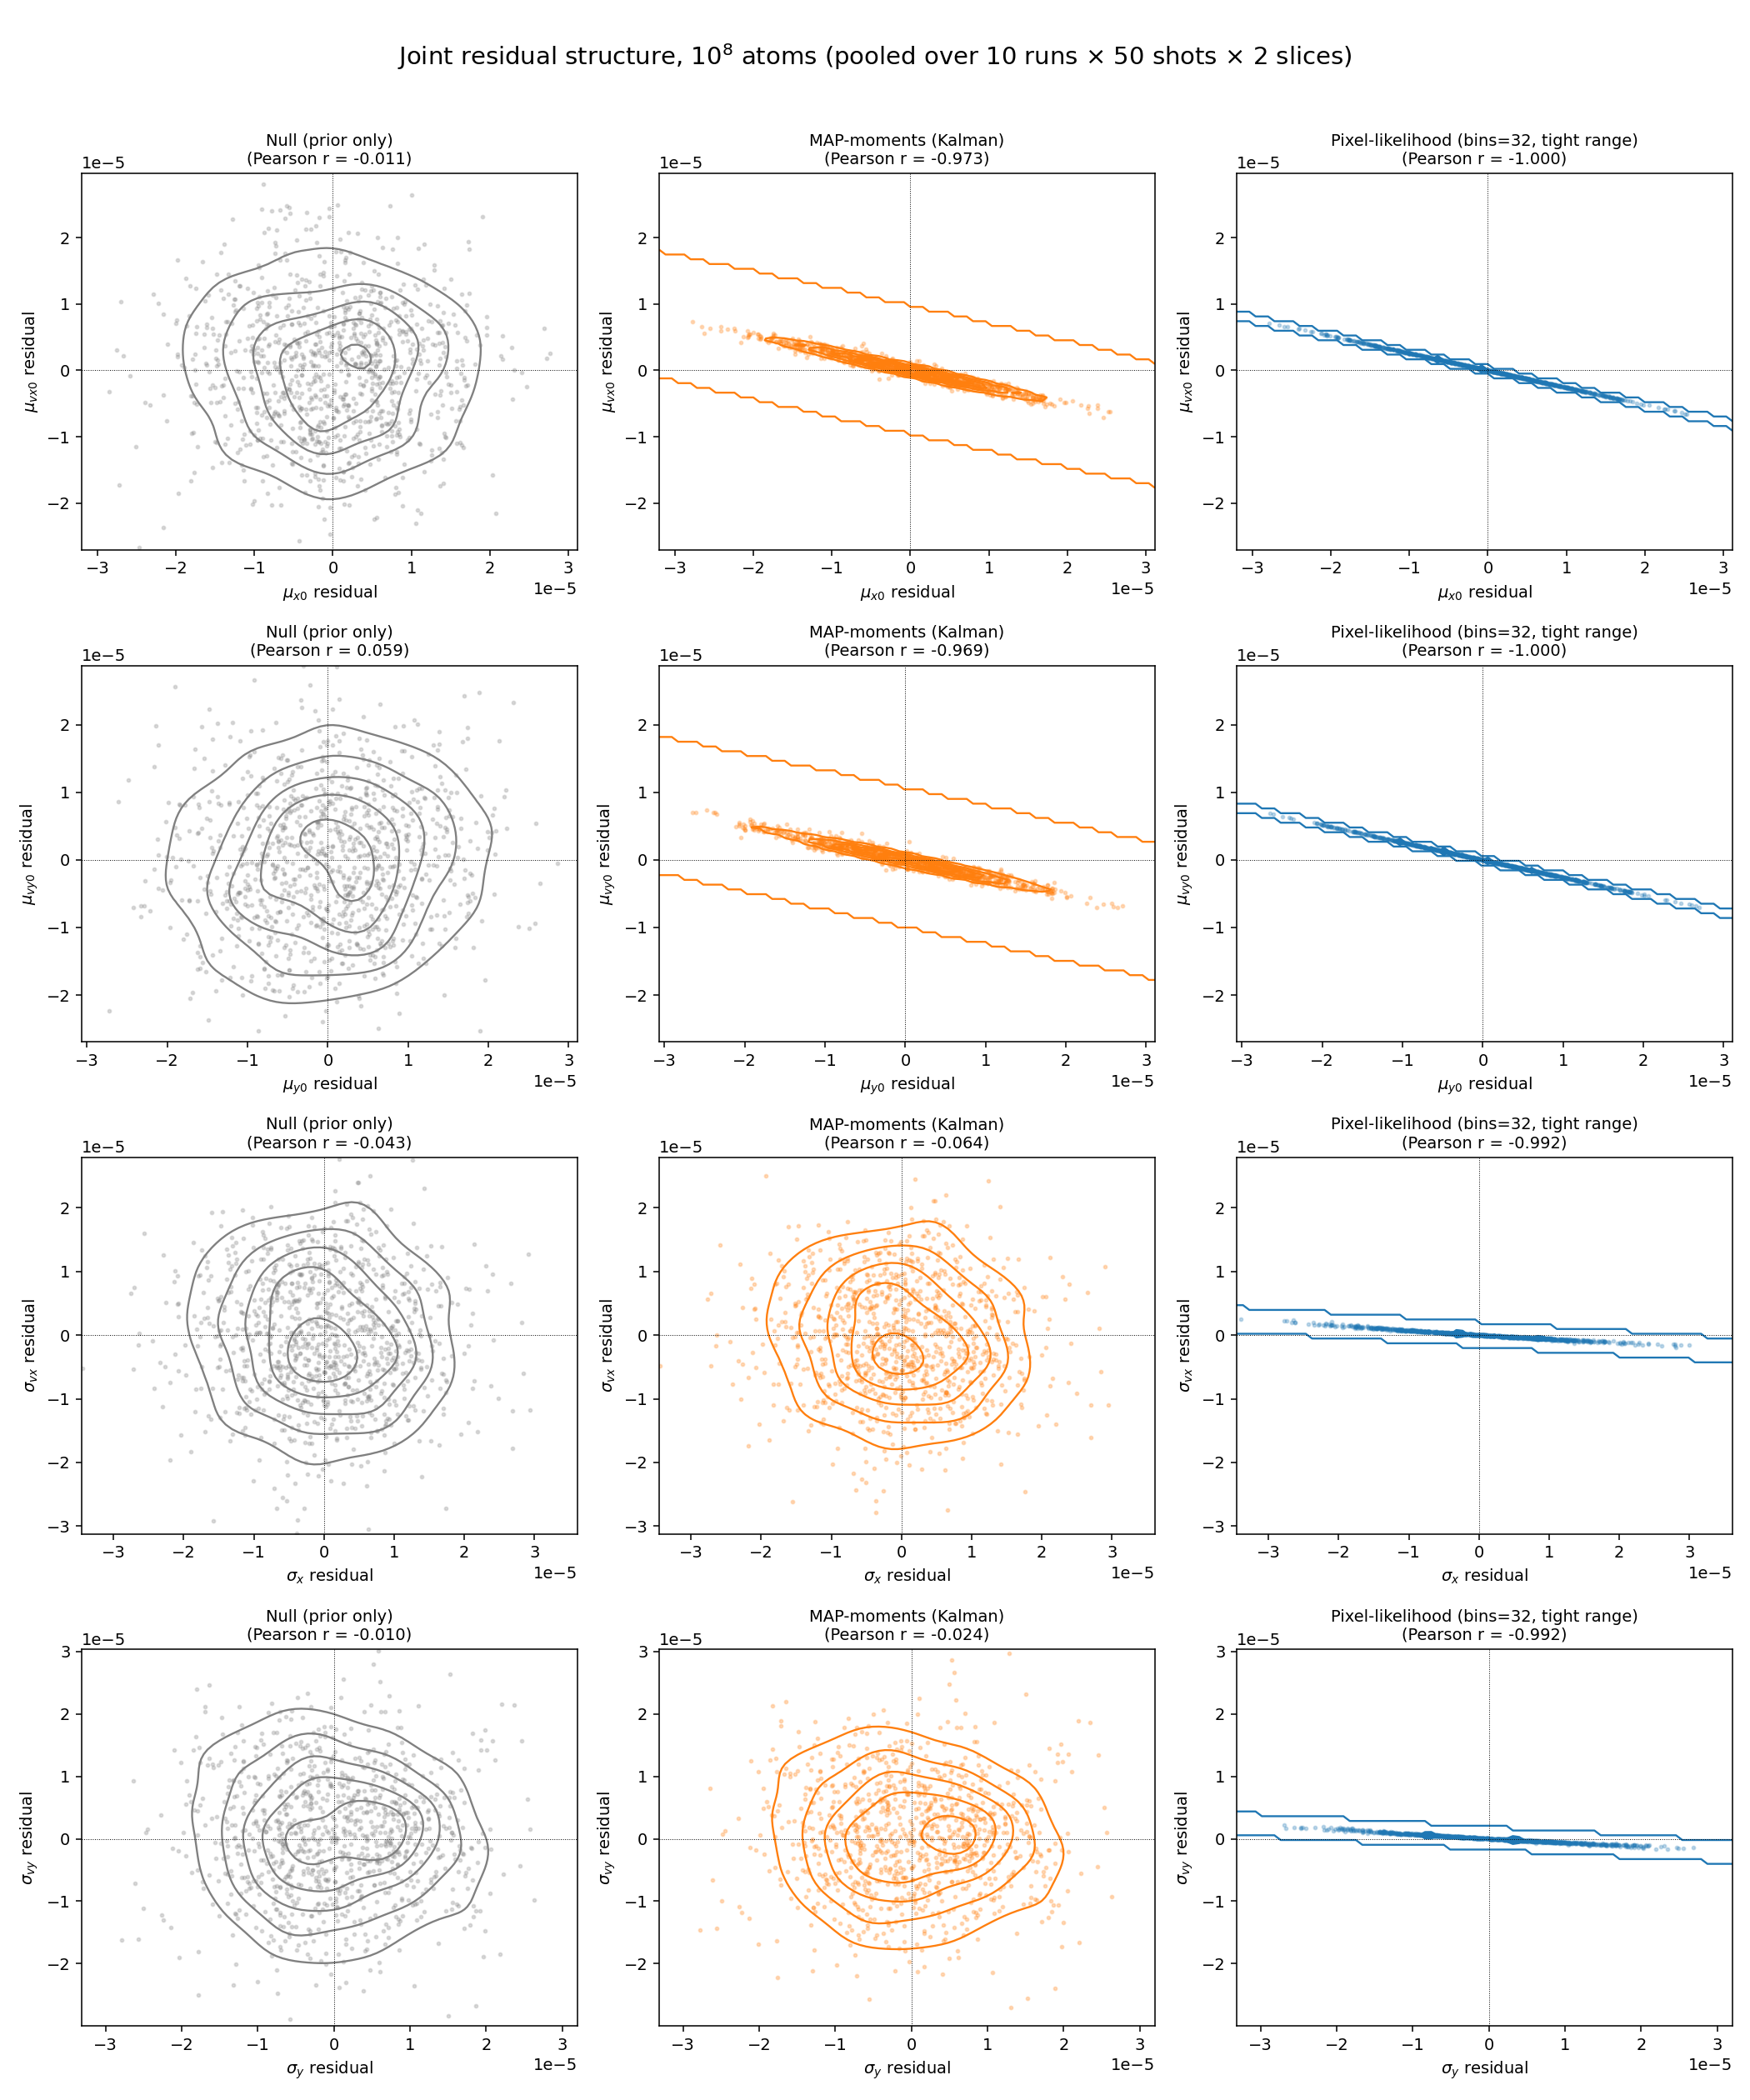
\includegraphics[width=\textwidth]{figures/residuals_2d_1e8.png}
  \caption{Joint residual structure for physically-coupled parameter pairs,
  $10^8$ atoms (see Appendix~\ref{sec:2dcorr} for the $10^6$-atom version,
  which shows the identical pattern). Density contours from a Gaussian KDE;
  points shown at 25\% opacity. Note the near-perfect anti-correlation for
  \emph{both} pairs for the pixel-likelihood method, vs.\ only the mean
  pair for moments.}
  \label{fig:res2d1e8}
\end{figure}

\subsection{Signal $(A_s,A_c)$ recovery}

Figure~\ref{fig:betascatter} shows $(\hat A_s,\hat A_c)$ for all 10
independent runs, by method and atom count. Table~\ref{tab:beta-rmse} gives
the RMSE.

\begin{figure}[htbp]
  \centering
  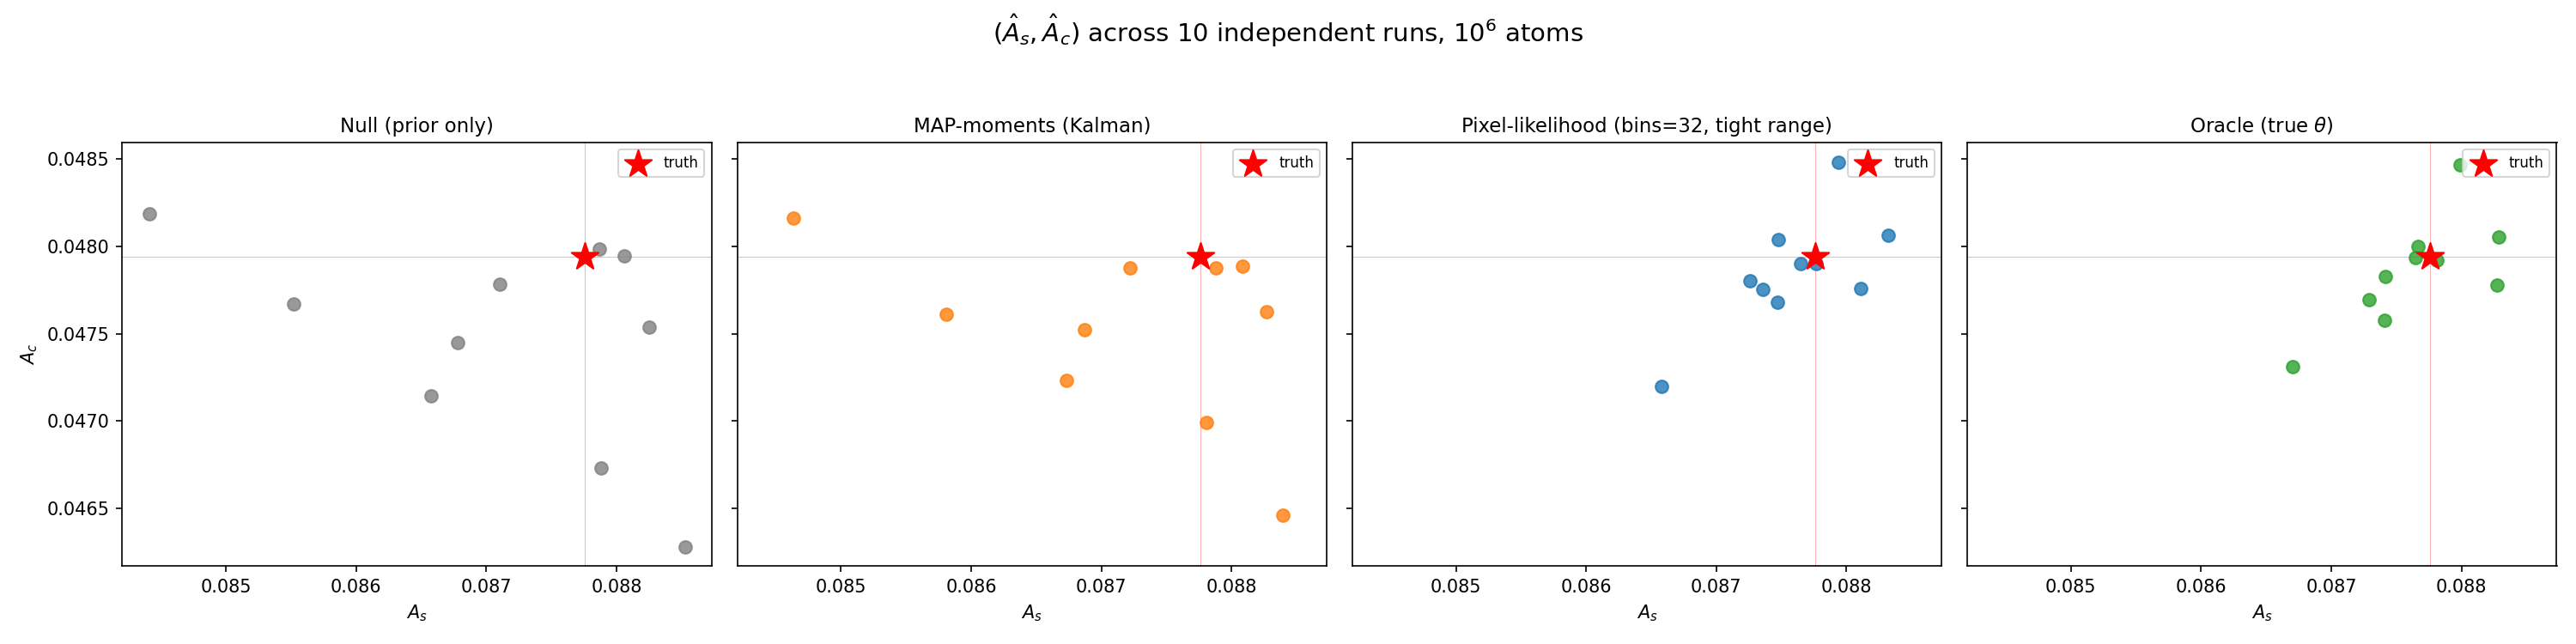
\includegraphics[width=\textwidth]{figures/beta_scatter_1e6.png}
  \\[6pt]
  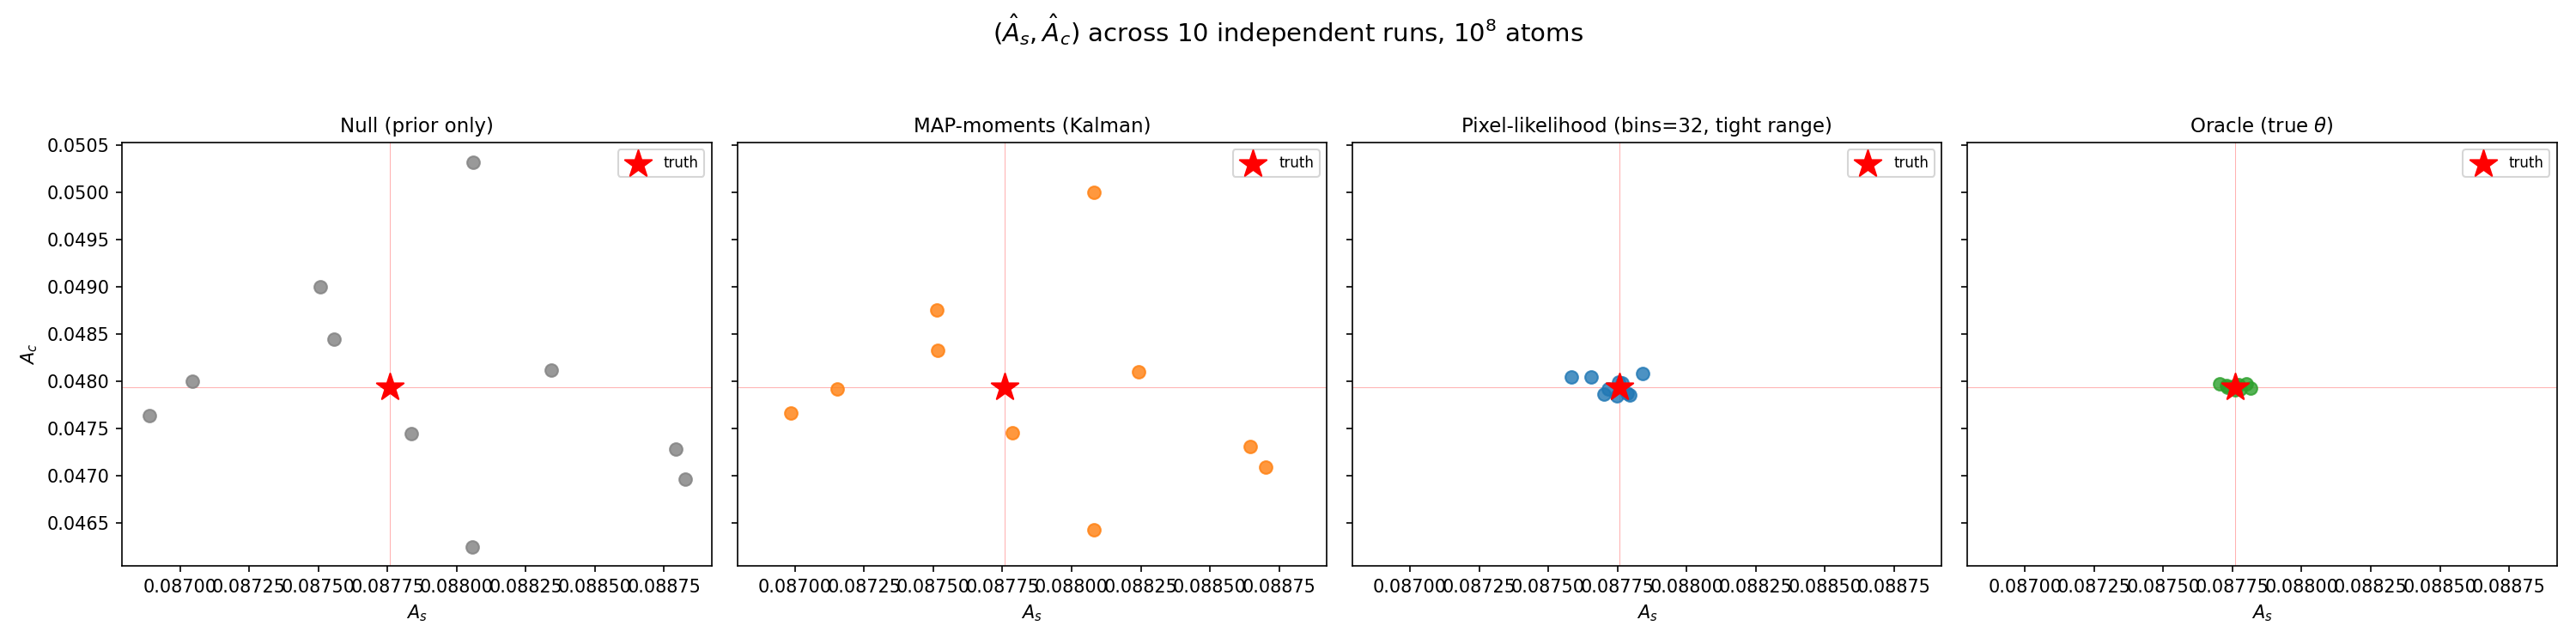
\includegraphics[width=\textwidth]{figures/beta_scatter_1e8.png}
  \caption{$(\hat A_s,\hat A_c)$ across 10 independent runs. Top: $10^6$
  atoms. Bottom: $10^8$ atoms. Note: axes are shared across the 4 panels
  within each row, so the visual tightening from null/moments to
  best/oracle is directly comparable.}
  \label{fig:betascatter}
\end{figure}

\begin{table}[htbp]
\centering
\caption{Signal $(A_s,A_c)$ RMSE by method and atom count, in mrad
($A_s,A_c$ are phase-modulation amplitudes: $\delta\phi_i(\beta)=A_s\sin(\cdot)+A_c\cos(\cdot)$
is a phase, Eq.~\ref{eq:dphi}, so $A_s,A_c$ carry the same units), $N=10$
independent runs.}
\label{tab:beta-rmse}
\begin{tabular}{lrrrr}
\toprule
& \multicolumn{2}{c}{$10^6$ atoms} & \multicolumn{2}{c}{$10^8$ atoms} \\
Method & RMSE($A_s$) [mrad] & RMSE($A_c$) [mrad] & RMSE($A_s$) [mrad] & RMSE($A_c$) [mrad] \\
\midrule
Null              & 1.412 & 0.737 & 0.641 & 1.078 \\
MAP-moments       & 1.284 & 0.636 & 0.566 & 0.936 \\
Pixel-likelihood (best) & $\mathbf{0.495}$ & $\mathbf{0.321}$ & $\mathbf{0.074}$ & $\mathbf{0.086}$ \\
Oracle            & 0.468 & 0.304 & 0.032 & 0.020 \\
\midrule
Best / moments ratio & 0.386 & 0.505 & 0.131 & 0.092 \\
Best / oracle ratio  & 1.058 & 1.056 & 2.31  & 4.30  \\
\bottomrule
\end{tabular}
\end{table}

%%============================================================
\section{Discussion}
\label{sec:discussion}
%%============================================================

\textbf{The kinematic-recovery advantage survives into a real, substantial
$\beta$-level improvement, and grows sharply with photon count.} At
$10^6$ atoms, the pixel-likelihood method beats the existing moment-based
estimator by $2.0$--$2.6\times$ in $\beta$ RMSE, and lands within $\sim\!6\%$
of the oracle (shot-noise) floor -- there is very little room left to
improve at this photon budget, consistent with earlier work in this project
finding \code{map\_inference.py} already close to its Cram\'er--Rao bound
at $10^6$ atoms. At $10^8$ atoms the picture changes qualitatively: moments
barely beats the uninformative null baseline (RMSE ratio $0.566/0.641=0.88$
on $A_s$), while the pixel-likelihood method is $7.6$--$10.9\times$ better
than moments and still has a genuine $2.3$--$4.3\times$ gap remaining to the
oracle floor -- i.e., at high photon count there is both a large amount of
information the moment method fails to extract, \emph{and} a large amount
the pixel-likelihood method (in its current, non-exhaustively-tuned
configuration) also leaves on the table.

\textbf{Why the effect is atom-count-dependent even though the kinematic
RMSE ratio (Table~\ref{tab:theta-rmse}) is not:} the $\sim\!12$--$13\times$
tightening of $\sigma_{vx},\sigma_{vy}$ is essentially constant across the
$100\times$ atom-count range, yet its effect on $\beta$ grows by
roughly $4$--$5\times$ from $10^6$ to $10^8$. This means the downstream
signal-fit step's \emph{sensitivity} to residual velocity-spread error, not
the size of that error itself, is what scales with photon count -- plausible
since more photons per shot let the signal-fit likelihood itself resolve
finer distinctions in the effective phase information, making it less
tolerant of a given absolute kinematic bias. This is stated as an
observation, not yet independently verified by a dedicated sensitivity
check.

\textbf{Caveats.} $N_{\rm RUNS}=10$ is a real but not huge sample -- the
$\beta$ RMSE numbers in Table~\ref{tab:beta-rmse} carry meaningful sampling
uncertainty of their own (not quantified here; a bootstrap or larger-$N$
re-run would tighten this). The pixel-likelihood configuration
(\code{bins=32}, tight range) was chosen by a hyperparameter search focused
on \emph{kinematic}-level RMSE (Appendix~\ref{sec:hp}), not by directly
optimising $\beta$-level RMSE -- the remaining oracle gap at $10^8$ atoms
suggests further gains may be available by pushing \code{bins} past 32 or
tuning the range cutoff more aggressively, not yet tested end-to-end through
the $\beta$-fit at this larger scale. Finally, all "best"-method fits used
the identical downstream $\beta$-fit configuration (\code{bins=16}, native
range, \code{gh\_order=12}) as the other three methods, by design
(\S\ref{sec:reduction}) -- so none of the reported gain comes from also
improving that shared step.

%%============================================================
\appendix
\section{Supporting Methodology}

\subsection{Joint residual structure at $10^6$ atoms}
\label{sec:2dcorr}

\begin{figure}[htbp]
  \centering
  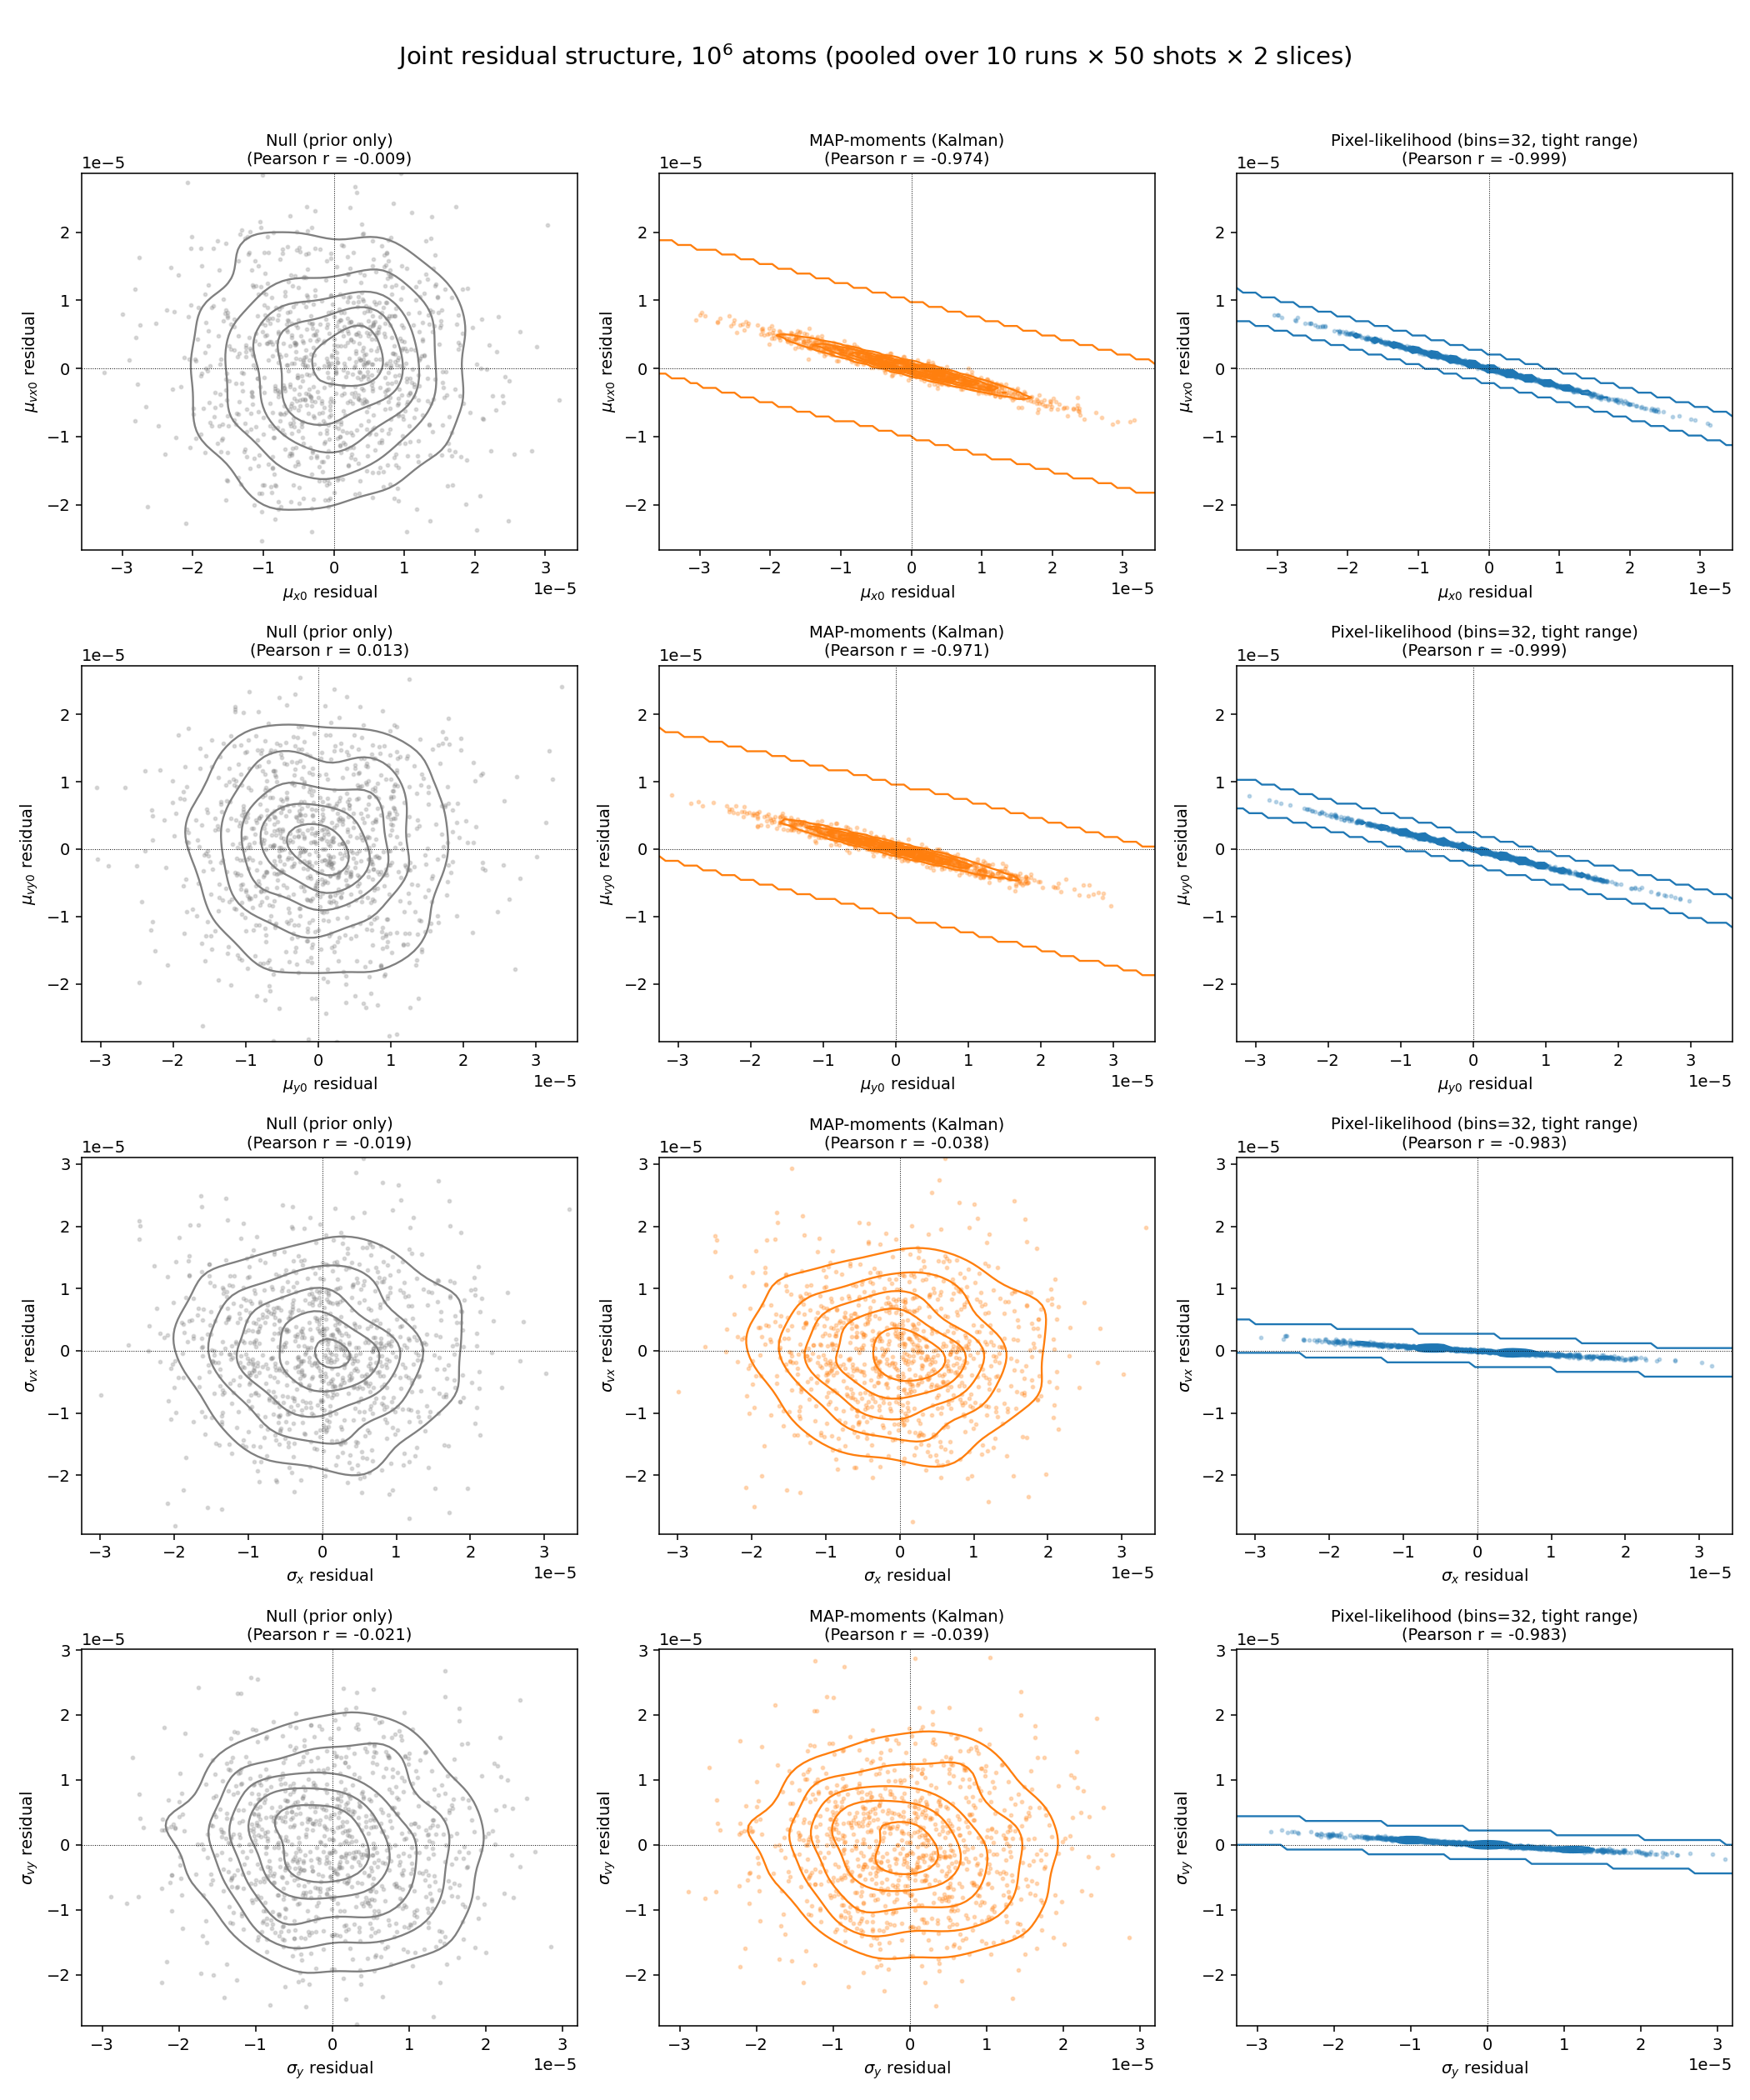
\includegraphics[width=\textwidth]{figures/residuals_2d_1e6.png}
  \caption{Joint residual structure (same pairs, same layout as
  Figure~\ref{fig:res2d1e8}), $10^6$ atoms. The correlation pattern
  discussed in \S\ref{sec:results} is essentially identical to the
  $10^8$-atom case.}
  \label{fig:res2d1e6}
\end{figure}

\subsection{Quadrature convergence for the $\phi$-marginal}
\label{sec:qconv}

The $\phi$-marginal integral (Eq.~\ref{eq:marginal-phi}) is evaluated on a
uniform grid of $M$ points over $[0,2\pi)$ via
\code{scipy.special.logsumexp} for numerical stability. $M$ was varied
from 500 to 8000 (on 3 independent test shots) and the resulting
$\hat\theta_{\rm MAP}$ tracked: it is stable to $\sim\!10^{-9}$ absolute
(against a parameter natural scale of $\sim\!10^{-5}$) already at $M=2000$,
which is the value used throughout this note.

\subsection{Tight-range derivation}
\label{sec:tightrange}

The dataset's native image half-range ($\pm3\,$mm) is set generously to
guarantee no clipping under worst-case cloud excursions, but the
\emph{bulk} of the photon flux occupies a much smaller region. Aggregating
photon counts vs.\ $|{\rm position}|$ across all 40 available runs (both
$10^6$ and $10^8$ atom datasets separately, giving consistent results:
$1.540\,$mm vs.\ $1.537\,$mm respectively) gives the following
flux-containment radii:

\begin{center}
\begin{tabular}{lrr}
\toprule
Fraction of total counts contained & half-range needed & ratio to native \\
\midrule
99\%     & $1.003\,$mm & $0.335$ \\
99.9\%   & $1.294\,$mm & $0.431$ \\
99.99\%  & $1.540\,$mm & $0.513$ \\
99.999\% & $1.762\,$mm & $0.587$ \\
\bottomrule
\end{tabular}
\end{center}

$99.99\%$ containment ($1.54\,$mm) was chosen: it loses only 1 photon in
$10^4$ (negligible relative to Poisson noise itself) while roughly halving
the pixel size at fixed \code{bins} -- i.e., a resolution improvement
essentially free of extra compute, since the number of bins (and hence the
model-evaluation cost) is unchanged; only the physical size each bin covers
shrinks.

\subsection{Hyperparameter sweep: bins vs.\ tight range, and whether they
compound}
\label{sec:hp}

Comparing \code{bins}$\in\{16,32\}$ crossed with \{native range, tight
range\} on the same 50-shot test set (velocity-spread RMSE, the parameters
where any effect is seen at all):

\begin{center}
\begin{tabular}{lrr}
\toprule
Configuration & RMSE($\sigma_{vx}$) [$\mu$m/s] & RMSE($\sigma_{vy}$) [$\mu$m/s] \\
\midrule
bins=16, native range (baseline)  & $0.869$ & $0.860$ \\
bins=32, native range             & $0.714$ & $0.663$ \\
bins=16, tight range              & $0.725$ & $0.681$ \\
bins=32, tight range (both)       & $0.699$ & $0.634$ \\
\bottomrule
\end{tabular}
\end{center}

The two do \emph{not} compound multiplicatively: combining both tricks
($0.805$/$0.737\times$ baseline) is only marginally better than either
alone ($0.821/0.771\times$ for bins=32; $0.835/0.792\times$ for tight
range), far short of the $\sim\!0.63$--$0.68\times$ a naive independent-effects
multiplication would predict. This indicates bins and range are tapping a
shared underlying resource (spatial resolution near the flux-dense region),
not two independent information sources, and that a real ceiling exists
around $\sim\!20$--$26\%$ improvement from spatial resolution alone at this
photon range. \code{bins=32} + tight range was used as "best" throughout
this note as the best-available combination, despite the modest marginal
gain over tight-range-alone, for consistency with the rest of the
investigation; a cost-sensitive deployment might prefer \code{bins=16} +
tight range for $\sim\!4\times$ lower compute at comparable quality.

\paragraph{A third bins value reveals the tight-range trick is not
universally beneficial.} Adding \code{bins=8} + tight range to the
comparison:

\begin{center}
\begin{tabular}{lrr}
\toprule
Configuration & RMSE($\sigma_{vx}$) [$\mu$m/s] & RMSE($\sigma_{vy}$) [$\mu$m/s] \\
\midrule
bins=16, native range (baseline)  & $0.869$ & $0.860$ \\
\textbf{bins=8, tight range}      & $\mathbf{0.955}$ & $\mathbf{0.962}$ \\
bins=16, tight range              & $0.725$ & $0.681$ \\
bins=32, tight range              & $0.699$ & $0.634$ \\
\bottomrule
\end{tabular}
\end{center}

At \code{bins=8}, tight range is \emph{worse} than the bins=16, native-range
baseline ($1.10\times$/$1.12\times$, i.e.\ a $\sim\!10\%$ regression) --
despite each pixel still being physically smaller in absolute terms
($0.385\,$mm vs.\ the native-range bins=8 pixel width of $0.75\,$mm). This
means the earlier framing (``tight range is essentially free and helps'')
is incomplete: it only helps once \code{bins} is already large enough to
exploit the freed-up resolution; at too few bins, whatever information is
lost by clipping the (mostly empty, but not perfectly empty) outer image
apparently outweighs the gain from finer pixel spacing. The bins=16$\to$32
trend genuinely flattens (a real, near-plateau ceiling, \S\ref{sec:hp}
above), but bins=8 is not on that same monotonic curve -- it is a
qualitatively worse regime, not merely a smaller improvement. Any future
attempt to push \code{bins} \emph{below} 16 with the tight-range trick
should not be assumed safe without re-checking this non-monotonicity.

\subsection{Semi-analytic gradient for the $\phi$-marginal, and why it was
necessary}
\label{sec:analytic-grad}

An initial attempt to estimate $\theta$'s local posterior curvature
(Hessian, for a Laplace-approximation uncertainty estimate) via finite
differences of the raw marginal NLL failed badly: the resulting Hessian had
negative eigenvalues and several exactly-zero implied variances, for a
majority of test shots, regardless of step-size tuning (fixed or adaptive).
The root cause: \emph{differentiating an already-approximate derivative}
-- \code{pixel\_acs\_grad.pixel\_acs\_and\_grad} itself computes $\theta$'s
gradient via an internal finite difference (\code{h\_theta=1e-9}), and a
second (outer) finite difference on top of that compounds numerical noise
in a way that step-size tuning could not reliably fix.

The fix: since $\phi$ only enters the model by combining $\theta$-dependent,
$\phi$-independent coefficients $(A,C^c,C^s)$ via $\cos\Phi,\sin\Phi$
(Eq.~\ref{eq:obs-model}), \code{pixel\_acs\_and\_grad} needs to be called
only \emph{once} per $\theta$ (already the case), and its returned
per-$\theta$-component gradient can be chained through the log-sum-exp
marginalisation analytically:
\begin{equation}
  \frac{\partial\,\text{marginal NLL}}{\partial\theta_k}
  = \sum_{m=1}^M w_m\,\frac{\partial\,\mathrm{NLL}(\theta,\phi_m)}{\partial\theta_k},
  \qquad w_m = \mathrm{softmax}_m\bigl(-\mathrm{NLL}(\theta,\phi_m)\bigr),
\end{equation}
i.e.\ a $\phi$-posterior-weighted average of the per-grid-point gradient --
no new finite differences introduced at the marginalisation step. This was
validated against a plain finite-difference gradient of the marginal NLL
at a fixed test point: relative agreement $\sim\!10^{-7}$--$10^{-4}$
component-wise, confirming correctness of the chain rule. Using this
gradient (\code{jac=True} in \code{scipy.optimize.minimize}) also
substantially speeds up the $\theta$-optimisation itself (converges in
$\sim\!6$ iterations vs.\ needing scipy's own finite-difference outer
gradient otherwise).

\end{document}
